\label{contexto}
El presente capítulo ofrece un análisis detallado del 
problema de la violencia y de las metodologías actuales 
para su detección en video, ambos aspectos fundamentales 
para el desarrollo de esta investigación. Se aborda la 
clasificación de los distintos tipos de violencia y su 
impacto a nivel global, así como una revisión exhaustiva 
de las soluciones más utilizados en la literatura para 
identificar eventos violentos en diferentes entornos.\\

La Sección \ref{contexto} establece una categorización de 
diversas formas de violencia, destacando su ocurrencia en 
diferentes contextos, como espacios públicos, entornos 
domésticos y situaciones de conflicto. Además, se presentan 
estadísticas relevantes que ilustran la magnitud del problema 
a nivel global, con un enfoque particular en América Latina 
y sus tendencias recientes. También se exponen las soluciones 
que se han utilizado para la detección y la toma de decisiones 
punitivas frente a los casos de violencia mencionados.\\

Por último, en la Sección \ref{estadodelarte} se revisan 
sistemáticamente los enfoques más representativos en la 
literatura para la detección de violencia en video utilizando 
inteligencia artificial. Cada metodología ha sido clasificada 
en función de su fundamento teórico y técnico, distinguiendo 
entre modelos basados en redes neuronales convolucionales 
(CNNs) y enfoques híbridos basados en \textit{pipelines}. 
Finalmente, se discute la necesidad de evaluar diferentes 
configuraciones de estos modelos para optimizar su rendimiento 
en la identificación de incidentes violentos.

\section{Contexto}\label{contexto}
Esta Sección presenta cada uno de los tipos de violencia 
clasificados por la OMS y cómo estos han afectado a la 
población a lo largo de los años. Además, se plantean de 
manera general cuáles han sido los enfoques o sistemas 
propuestos para combatirlos.\\

La proliferación de la violencia en todo el mundo constituye 
un problema social creciente que afecta la convivencia y el 
sentido de seguridad entre las personas. Dependiendo de las 
características de quienes cometen el acto, la violencia 
puede clasificarse en las siguientes categorías \cite{OMS2014}:
 
\begin{itemize} 
    \item Autoinfligida (conducta suicida y autolesiones), 
    \item Interpersonal (violencia doméstica, incluyendo a niños, 
    parejas y personas mayores; así como violencia entre personas 
    no relacionadas), 
    \item Colectiva (social, política y económica). 
\end{itemize}

La OMS clasifica los actos de violencia según su naturaleza como: 
física, sexual, psicológica, privación y negligencia. 
Con base en datos de 2014, indicó que ``los actos 
repetidos de violencia que van desde la intimidación, el acoso 
sexual y las amenazas hasta la humillación y el menosprecio de 
los trabajadores pueden convertirse en casos muy graves debido 
al efecto acumulativo. En Suecia, se estima que dicho 
comportamiento ha sido uno de los factores más importantes en el 
10\% al 15\% de los suicidios''. \\

En el mismo documento se menciona que, en el año 2000, hubo 
alrededor de 199,000 homicidios de jóvenes en todo el mundo 
(9.2 por cada 100,000 habitantes). Es decir, en promedio, 
mueren diariamente 565 niños, adolescentes y adultos jóvenes, 
de entre 10 y 29 años, como resultado de la violencia 
interpersonal. Las tasas de homicidio varían considerablemente 
según la región, desde 0.9 por cada 100,000 habitantes en 
países de altos ingresos en Europa y algunas partes de Asia 
y el Pacífico, hasta 17.6 en África y 36.4 por cada 
100,000 en América Latina.\\

Por otro lado, el informe del Fondo Monetario Internacional 
revela un aumento exponencial en la sensación de inseguridad y 
una mayor aceptación de que los crímenes violentos son, 
unánimemente, el problema más importante desde 2020, como 
se muestra en la Figura \ref{fig:percepcion} \cite{Bisca2024}:\\

\begin{figure}[h!] 
    \centering
    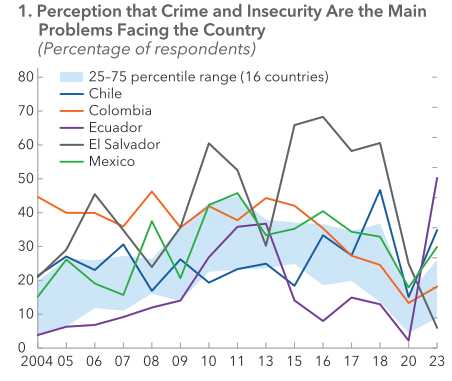
\includegraphics[width=0.7\textwidth]{images/inseguridad2024.png} % Adjust the width and file path
    \caption[Percepción que la inseguridad como una prioridad nacional]
    {Percepción que la inseguridad como una prioridad nacional \protect \cite{Bisca2024}}
    \label{fig:percepcion}
\end{figure}

La Figura \ref{fig:percepcion} muestra las prioridades en función 
del tiempo de la población en diferentes países latinoamericanos. 
La percepción de la violencia como prioridad venía disminuyendo 
desde 2004; sin embargo, en los últimos cinco años, esta 
percepción ha mostrado una tendencia marcadamente creciente.\\

En este contexto, la vigilancia y la intervención temprana se 
han convertido en herramientas clave para prevenir hechos 
violentos y proteger a las posibles víctimas. 
Tradicionalmente, los mecanismos de vigilancia han dependido 
de recursos humanos, como la observación directa a través de 
cámaras por parte del personal de seguridad. Actualmente, 
existen soluciones más automatizadas basadas en inteligencia 
artificial (IA), la cual ha emergido como una alternativa 
prometedora para automatizar el proceso de vigilancia, 
ofreciendo herramientas más rápidas, escalables y precisas 
para identificar comportamientos anómalos.\\

En la sección \ref{solucionesClásicas} se presentan las 
soluciones que se han aplicado desde tiempos antiguos, 
las cuales consistían mayormente en el uso de la policía 
o milicia para el apaciguamiento y la reacción ante 
incidentes violentos, así como en la planificación de la 
seguridad residencial a través de reportes policiales 
y ciudadanos. \\

Por otra parte, en la sección \ref{solucionesTecnologicas} se 
presentarán las mejoras a los sistemas mencionados anteriormente 
utilizando soluciones tecnológicas basados en métodos estadísticos.

\subsection{Soluciones Clásicas}\label{solucionesClásicas}

Desde la antigüedad, los estados han utilizado la organización 
militar como principal herramienta para contener la violencia 
interna y establecer el orden. En imperios como el romano o 
el chino, los soldados eran distribuidos estratégicamente en 
territorios clave, no solo para la defensa externa, sino 
también para prevenir revueltas, aplicar justicia y garantizar 
la autoridad del Estado \cite{Gilliver2005}. Estas asignaciones 
eran determinadas por el mando central según criterios 
geográficos, demográficos y políticos, pero siempre con una 
intención clara: imponer un monopolio legítimo de la fuerza, 
siguiendo lo que Max Weber definiría siglos después como una 
característica esencial del Estado moderno.\\

A partir del siglo XIX, con la consolidación de cuerpos 
policiales profesionales en Europa y América, surgieron 
modelos más especializados para combatir la violencia 
interna, especialmente en contextos urbanos en crecimiento. 
Las asignaciones de personal policial se realizaban mediante 
mapas manuales de criminalidad, análisis de denuncias y 
supervisión directa, con el objetivo de prevenir delitos, 
desarticular disturbios y pacificar zonas consideradas 
conflictivas \cite{Emsley2007}. Sin embargo, estas asignaciones 
dependían en gran medida de la interpretación subjetiva 
de los mandos y, en muchas ocasiones, respondían a presiones 
políticas o sesgos institucionales, lo que afectaba 
su efectividad en la reducción sostenible de la violencia.\\

Hasta inicios de los años 1990, tanto en contextos militares 
como policiales, la distribución de fuerzas para combatir 
la violencia interna se realizaba sin apoyo computacional, 
lo que limitaba la capacidad para prever patrones delictivos 
o reasignar recursos de manera eficiente. La planificación 
se basaba en documentos físicos, experiencia de campo y 
órdenes jerárquicas, lo cual implicaba lentitud en la 
respuesta y escasa adaptación al cambio \cite{sheptycki1998}. 
Esta rigidez estructural dificultaba la aplicación de 
estrategias preventivas a largo plazo y, en muchas ocasiones, 
resultaba en una gestión reactiva de la violencia, en lugar 
de su erradicación sistemática o de un abordaje desde 
perspectivas más integrales. \\

\subsection{Soluciones tecnológicas}\label{solucionesTecnologicas}

La presente sección expone algunos de los sistemas implementados 
para solucionar las ineficiencias subjetividad de las soluciones 
clásicas para este problema. Para ello, se utilizaron enfoques 
más basados en datos estadísticos para su implementación. 

El primer sistema de vigilancia fue creado en la década de 
1960, inicialmente en Londres, Reino Unido, como una 
estrategia para monitorear el tráfico. Sin embargo, en los 
años 1990, su propósito se expandió al control del crimen y 
la violencia urbana. Las cámaras de circuito cerrado de 
televisión (CCTV) fueron instaladas en zonas de alto riesgo, 
estaciones de tren, centros comerciales y calles céntricas, con 
el objetivo de disuadir actos violentos, registrar evidencia 
visual de delitos y mejorar la capacidad de respuesta de las 
fuerzas policiales. A diferencia de las tecnologías modernas 
que dependen de IA para el análisis automático, estos 
sistemas tradicionales requieren monitoreo humano en centros 
de control y revisión manual de grabaciones \cite{Vilalta2019}.\\

Uno de los primeros sistemas analíticos fue CompStat, 
desarrollado por la policía de Nueva York en 1994 para mejorar 
la eficacia en la respuesta policial al crimen. Este sistema 
basado en datos permite analizar tendencias delictivas mediante 
la recopilación y distribución de estadísticas. CompStat no 
solo mejora la respuesta ante la violencia, sino que también 
asigna recursos eficientemente, identifica patrones delictivos y 
ajusta estrategias en tiempo real. La combinación de datos 
y reuniones periódicas con líderes policiales facilita una 
supervisión directa y una rendición de cuentas más efectiva 
\cite{perf2003compstat}.\\

Tras su implementación en Nueva York, CompStat fue adoptado 
por diversas agencias policiales en Estados Unidos y otras 
partes del mundo \cite{weisburd2003reforming}. Su enfoque 
basado en datos ha permitido reducir la violencia en algunas 
de las ciudades más grandes del país, como Los Ángeles y 
Chicago. Además de aplicarse en crímenes violentos, el 
sistema ha demostrado ser efectivo para mejorar la eficiencia 
operativa, permitiendo a las fuerzas de seguridad adaptar 
rápidamente sus tácticas ante la dinámica cambiante delictiva. 
El éxito de CompStat ha impulsado su integración con otras 
soluciones de análisis de datos y monitoreo, convirtiéndose 
en una herramienta clave para la reducción del crimen a nivel 
mundial.\\

Otra solución más reactiva fue el Botón de pánico en México, 
un dispositivo diseñado para brindar seguridad inmediata en 
situaciones de violencia \cite{cdmx2008botonpanico}. Permite 
a las víctimas, ya sea en el hogar o en la vía pública, 
enviar una señal de alerta a autoridades o familiares con 
solo presionar un botón. Puede estar integrado en un móvil 
o en un aparato independiente que envía un mensaje con la 
ubicación exacta del usuario, facilitando una respuesta rápida, 
por ejemplo, desde un poste. Aunque surgió en México, se 
ha implementado en varios países de América Latina como parte 
de sus políticas públicas de seguridad.\\

En El Salvador, el Sistema de Alerta Temprana, desarrollado 
en 2012, monitorea y alerta sobre incidentes violentos, 
especialmente relacionados con pandillas y crimen organizado. 
Recoge datos de diversas fuentes, como reportes ciudadanos, 
medios, redes sociales y bases oficiales. Permite 
identificar riesgos y patrones de violencia antes de que se 
conviertan en amenazas graves. Destaca por generar alertas 
en tiempo real, facilitando que las autoridades tomen medidas 
preventivas antes de que ocurran actos violentos 
\cite{MinisteriodeJusticiaySeguridadPblica2025}.\\

Existen muchas más implementaciones tecnológicas como 
las detalladas anteriormente, las cuales, en su mayoría, 
son soluciones preventivas o reactivas que presentan cierta 
subjetividad o demora en la detección de actos violentos a 
nivel mundial. Para tratar de optimizar estos problemas, en 
los últimos años se ha decidido incorporar el uso de 
inteligencia artificial a las soluciones existentes. \\

\section{Estado del arte}\label{estadodelarte}

Para lograr comprender cómo funcionan las propuestas que 
han hecho uso de la inteligencia artificial en la actualidad, 
es necesario primero entender cómo funciona esta nueva 
tecnología.

La sección \ref{cnn} se explica la arquitectura de las 
\textit{Convolutional Neural Networks} (CNN) consistiendo en 
modelos basados en capas convolucionales para la extracción de 
características, clasificación y regresión de entradas matriciales 
como imágenes. 

La sección \ref{rnn} y la sección \ref{lstm} presentan arquitecturas 
especializadas para el procesamiento de datos sequenciales. Estas 
arquitecturas permiten realizar la clasificación o regresión de dichos 
datos secuenciales para hacer \textit{forecasting} d los datos para 
predicciones futuras. 

La sección \ref{transformer} presentan a los \textit{transformers} 
término que representa a una arquitectura 
con capas de autoatención de los datos que actualmente representan 
el estado del arte para muchas aplicaciones, tales como visión 
computacional, regresión, clasificación, procesamiento de lenguaje 
natural, etc.

La sección \ref{sba} habla de los algoritmos basados en esqueleto 
humano, el cual permite mapear movimientos complejos del cuerpo 
humano.

\subsection{\textit{Convolutional Neural Networks} (CNN)}\label{cnn}

Las CNN son modelos basados en una arquitectura diseñada 
específicamente para el análisis de imágenes, en particular 
para tareas de clasificación. Estas redes realizan la 
extracción de características mediante operaciones de 
convolución, lo que evita la pérdida de información y mejora 
tanto la eficiencia como la precisión respecto a arquitecturas 
anteriores \cite{Goodfellow-et-al-2016}.\\

Las convoluciones se basan en un procedimiento que extrae 
características mediante la aplicación de una pequeña matriz 
de transformación cuadrada sobre la imagen original, generando 
una versión modificada de esta. Dichas matrices de transformación 
se conocen como kernels \cite{Lecun2015}. La Figura 
\ref{convolucion} ilustra una iteración del proceso de 
convolución.\\

\begin{figure}[h!] 
    \includegraphics[width=0.7\textwidth]{images/convolución.png} 
    \centering 
    \caption[Proceso simplificado de una convolución]
    {Proceso simplificado de una convolución\protect \cite{convoluciones}.}
    \label{convolucion} 
\end{figure}

Por otro lado, existen otras capas fundamentales conocidas como 
\textit{poolings}. Estas 
capas aplican una operación específica sobre un cuadrante de la 
matriz resultante de las convoluciones. La lógica utilizada 
depende de los objetivos del modelo y las necesidades del 
usuario \cite{pooling}. La Figura \ref{pooling} compara dos 
tipos comunes: \textit{Max Pooling} y \textit{Average Pooling}, 
los cuales obtienen respectivamente el valor máximo y el 
promedio de cada cuadrante, generando así una nueva representación 
con menor dimensionalidad.\\

\begin{figure}[h!] 
    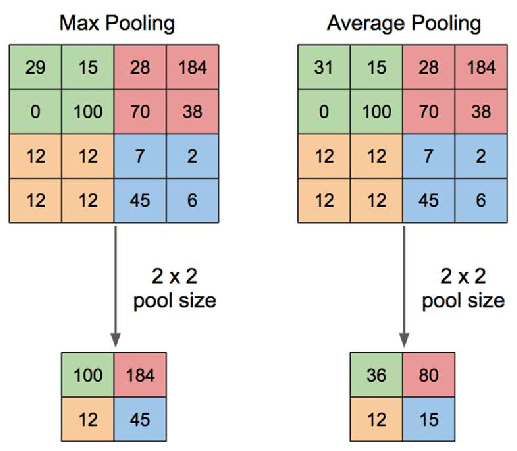
\includegraphics[width=0.6\textwidth]{images/pooling.png} 
    \centering 
    \caption[Proceso simplificado de un pooling]
    {Proceso simplificado de un pooling \protect \cite{pooling}.}
    \label{pooling} 
\end{figure}

Las CNN están formadas por combinaciones repetidas de capas 
convolucionales y de pooling, culminando en un conjunto de capas 
densas conocidas como Multi Layer Perceptron (MLP), encargadas 
del procesamiento final de las características extraídas 
\cite{Goodfellow-et-al-2016}. La Figura \ref{CNN} ilustra 
la estructura de una CNN. Como se mencionó anteriormente, la 
extracción de características se lleva a cabo dentro de la 
propia red, lo que evita la pérdida de información común en 
los MLP cuando se utilizan de forma aislada, dejando a estos 
últimos únicamente la tarea de clasificación.\\

\begin{figure}[h!] 
    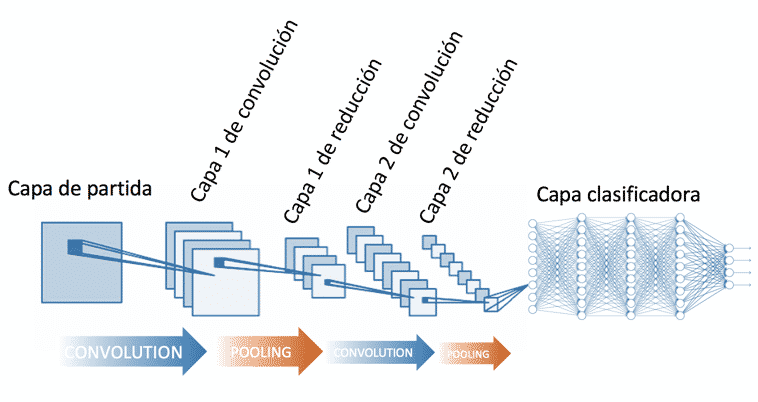
\includegraphics[width=1\textwidth]{images/CNN.png} 
    \centering 
    \caption[Arquitectura de una CNN convencional ]
    {Arquitectura de una CNN convencional \protect \cite{CNN-Arquitectura}.}
    \label{CNN} 
\end{figure}

La Figura \ref{CNN} mostrada anteriormente es un ejemplo muy pequeño 
comparado con las CNN del estado del arte que se presentarán en 
secciones siguientes, pero refleja la arquitectura que comparten la 
mayoría de ellas.


\subsection{\textit{Recurrent Neural Networks} (RNN's)}\label{rnn}

Las redes neuronales recurrentes (RNN, por sus siglas en 
inglés) son un tipo de arquitectura de red neuronal diseñada 
para procesar secuencias de datos, como texto, señales de 
audio o series temporales. A diferencia de las redes neuronales 
tradicionales (\textit{feedforward}), las RNNs cuentan con conexiones 
cíclicas que permiten que la información persista en el 
tiempo, lo cual es fundamental para modelar dependencias 
temporales o contextuales. En su forma básica, una RNN 
toma una entrada secuencial y actualiza un estado oculto 
interno a cada paso, el cual captura información de entradas 
previas. Este estado oculto actúa como una "memoria" 
dinámica que se transmite a través del tiempo, lo que hace 
posible que la red utilice información pasada para influir 
en las decisiones presentes \cite{elman1990finding}. La 
arquitectura simplificada se ilustra en la Figura \ref{image:RNN}.

\begin{figure}[h!] 
    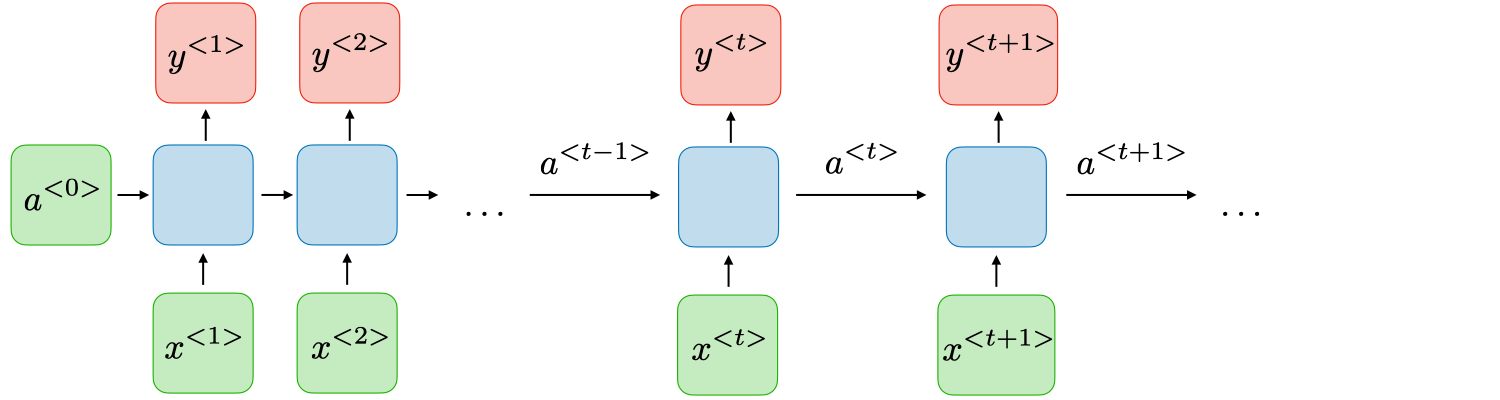
\includegraphics[width=1\textwidth]{images/RNN.png} 
    \centering 
    \caption[Versión simplificada de RNN.]
    {Versión simplificada de RNN \protect \cite{Aslam2019}.}
    \label{image:RNN} 
\end{figure}

Sin embargo, las RNN tradicionales enfrentan limitaciones 
prácticas debido al problema del desvanecimiento o explosión 
del gradiente, lo cual dificulta el aprendizaje de relaciones 
a largo plazo dentro de la secuencia. A pesar de estas 
limitaciones, las RNNs han sido fundamentales en el 
desarrollo de modelos secuenciales y han servido de base para 
arquitecturas más complejas como LSTM (\textit{Long Short-Term Memory}) 
y GRU (\textit{Gated Recurrent Units}), que fueron diseñadas para 
mitigar estos problemas. La formulación moderna de las RNNs 
fue introducida por 1990 \cite{elman1990finding}, 
quien propuso una red simple que puede aprender 
representaciones temporales a partir de datos secuenciales 
mediante el uso de retroalimentación interna en la 
arquitectura.

\subsection{\textit{Long Short-Term Memory} (LSTM)}\label{lstm}

Las redes \textit{Long Short-Term Memory} (LSTM) fueron 
desarrolladas como una extensión de las redes neuronales 
recurrentes (RNN) con el propósito de superar la dificultad 
de aprender dependencias a largo plazo en secuencias
 \cite{hochreiter1997lstm}. Las 
RNN tradicionales tienden a sufrir del problema del 
desvanecimiento o explosión del gradiente durante el 
proceso de entrenamiento, lo que limita su capacidad 
para capturar relaciones temporales distantes. Las LSTM 
abordan esta limitación mediante la incorporación de una 
memoria interna controlada por compuertas, lo que permite 
conservar información relevante a lo largo del tiempo.\\

La arquitectura de las LSTM se basa en una celda de memoria 
capaz de mantener su estado a lo largo de múltiples pasos 
temporales. Esta celda está regulada por tres compuertas 
fundamentales: la compuerta de entrada, que controla qué 
nueva información se almacena en la celda; la compuerta 
de olvido, que decide qué información debe eliminarse 
del estado anterior; y la compuerta de salida, que 
determina qué parte del contenido de la celda se utiliza 
como salida. Estas compuertas permiten que la red aprenda a 
retener o descartar información de manera adaptativa, mejorando 
significativamente el aprendizaje de secuencias largas.\\

Gracias a esta estructura, las LSTM han demostrado un 
rendimiento notable en una amplia gama de tareas secuenciales 
donde el contexto temporal es esencial. Aplicaciones como 
el modelado del lenguaje natural, la traducción automática, 
el reconocimiento de voz y el análisis de series temporales 
se han beneficiado enormemente de su capacidad para capturar 
dependencias a largo plazo. En consecuencia, las LSTM se han 
convertido en una arquitectura fundamental dentro del campo 
del aprendizaje profundo secuencial. La arquitectura de este 
modelo se puede ver en la Figura \ref{lstm}.

\begin{figure}[h!] 
    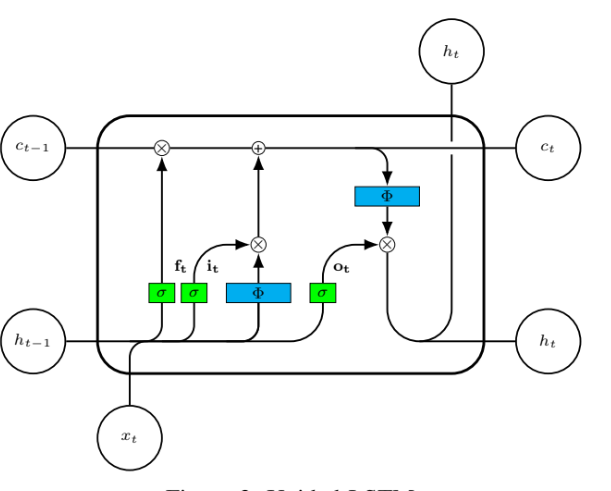
\includegraphics[width=1\textwidth]{images/lstm.png} 
    \centering 
    \caption[Representación de la arquitectura de LSTM.]
    {Representación de la arquitectura de LSTM\protect \cite{Orozco2021}.}
    \label{lstm} 
\end{figure}

\subsection{Transformers} \label{transformer}

Los transformers son una arquitectura de redes neuronales 
introducida en 2017 \cite{vaswani2017attention}, 
originalmente diseñada para tareas de procesamiento de 
lenguaje natural. Su principal innovación es el mecanismo 
de autoatención (\textit{self-attention}), 
que permite al modelo identificar qué partes de una secuencia 
son más relevantes entre sí, sin depender del orden 
secuencial como ocurre en RNNs. Este mecanismo proyecta las 
entradas en vectores de consulta (Q), clave (K) y valor (V), 
y calcula sus relaciones mediante un producto punto escalado, 
permitiendo capturar dependencias contextuales a largo plazo. 
Además, se introducen codificaciones posicionales para 
preservar el orden de los datos, y se utiliza atención 
multi-cabeza (\textit{multi-head attention}) para que el modelo pueda 
aprender diversas relaciones de atención de manera paralela. 
Esta estructura permite un entrenamiento más eficiente y una 
mejor capacidad de generalización. Esto se puede evidenciar en 
la Figura \ref{Image:transformer}.

\begin{figure}[h!] 
    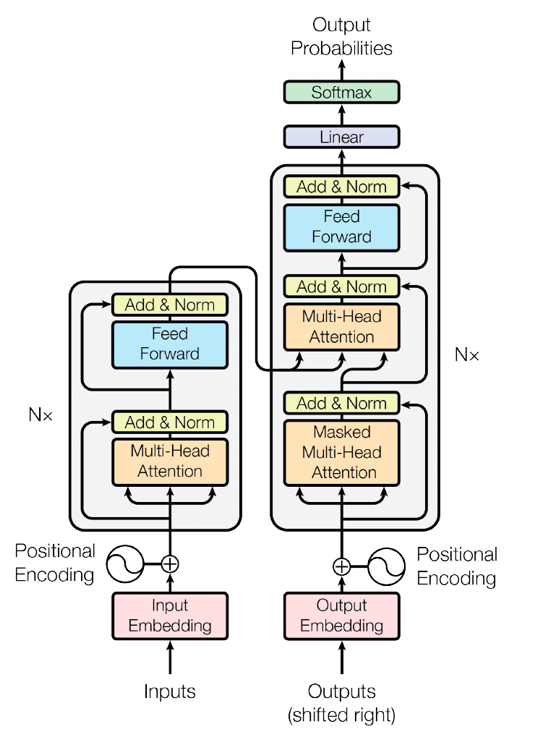
\includegraphics[width=1\textwidth]{images/transformer.png} 
    \centering 
    \caption[Representación de la arquitectura de un transformer.]
    {Representación de la arquitectura de un transformer\protect \cite{vaswani2017attention}.}
    \label{Image:transformer} 
\end{figure}

Aunque su uso inicial fue en lenguaje natural, los 
transformers fueron adaptados para clasificación de imágenes 
mediante el modelo textit{Vision Transformer} (ViT) \cite{Dosovitskiy2020}. 
En lugar de procesar secuencias de palabras, las imágenes se dividen en 
parches (por ejemplo, de 16x16 píxeles), que luego son 
linealmente proyectados a vectores y tratados como si fueran 
``palabras'' en una secuencia. A estos vectores se les 
suman codificaciones posicionales, y se procesan con la 
arquitectura transformer para capturar relaciones espaciales 
entre los distintos parches. Al finalizar las capas de 
atención, se utiliza un token de clase (similar al [CLS] 
en NLP) que se conecta a una capa densa para realizar la 
predicción de clase. Esta aproximación ha demostrado 
resultados competitivos con arquitecturas CNN tradicionales, 
y ha abierto nuevas líneas de investigación para aplicar 
transformers a tareas visuales de manera generalizada.

\subsection{Algoritmos basados en la captura esquelética (SBA)}
\label{sba}

Los algoritmos basados en esqueletos (\textit{skeleton-based}) 
para el reconocimiento de acciones humanas utilizan datos 
tridimensionales de las articulaciones del cuerpo humano 
para identificar y clasificar actividades \cite{LoPresti2016}. Estos datos se 
obtienen mediante sensores de profundidad, como Microsoft 
Kinect, o a través de técnicas de estimación de pose en 
imágenes RGB. Una vez capturados, los datos esqueléticos se 
procesan para modelar la estructura y el movimiento del 
cuerpo humano, permitiendo a los algoritmos aprender patrones 
temporales y espaciales asociados a diferentes acciones. 
Este enfoque ofrece ventajas significativas, como la 
reducción de la influencia de factores externos como la 
iluminación o el fondo, y proporciona una representación más 
abstracta y robusta del movimiento humano.

El reconocimiento de acciones basado en esqueletos ha 
evolucionado con el tiempo, incorporando diversas arquitecturas 
de aprendizaje profundo para mejorar su precisión y 
eficiencia \cite{Ren2024}. Entre las técnicas más destacadas se encuentran 
las redes neuronales recurrentes (RNNs), que capturan la 
dinámica temporal de las secuencias de movimiento; las 
redes neuronales convolucionales (CNNs), que extraen 
características espaciales; y las redes de convolución en 
grafos (GCNs), que modelan las relaciones estructurales entre 
las articulaciones del cuerpo. Estas arquitecturas permiten 
a los sistemas aprender representaciones complejas de las 
acciones humanas, mejorando su capacidad para reconocer 
actividades en diversos contextos y condiciones.


\subsection{Consideraciones}

Cada una de las arquitecturas anteriormente mencionadas tiene 
cierta utilidad con respecto a su estructura. La Tabla
\ref{tabla:comparativa} hace un resumen con respecto a 
las características de cada arquitectura.

\begin{table}[h]
\centering
\footnotesize
\caption{Tabla comparativa de arquitecturas para detección de violencia.}
\begin{tabular}{|l|c|c|c|c|}
\hline
\multicolumn{1}{|c|}{\textbf{}}                                                     & \textbf{CNN}                                                                                            & \textbf{LSTM}                                                                                            & \textbf{Transformers}                                                                                       & \textbf{SBA}                                                                                                     \\ \hline
\textbf{\begin{tabular}[c]{@{}l@{}}Tipo de \\ datos\end{tabular}}                   & \begin{tabular}[c]{@{}c@{}}Datos \\ espaciales \\ (imágenes)\end{tabular}                               & \begin{tabular}[c]{@{}c@{}}Datos \\ secuenciales\\ largos\end{tabular}                                   & \begin{tabular}[c]{@{}c@{}}Datos \\ secuenciales \\ paralelizables\end{tabular}                             & \begin{tabular}[c]{@{}c@{}}Coordenadas de \\ articulaciones \\ humanas (3D o 2D)\end{tabular}                    \\ \hline
\textbf{\begin{tabular}[c]{@{}l@{}}Entrada \\ esperada\end{tabular}}                & \begin{tabular}[c]{@{}c@{}}Imágenes, \\ video \\ (por frame)\end{tabular}                               & \begin{tabular}[c]{@{}c@{}}Secuencias \\ largas\end{tabular}                                             & \begin{tabular}[c]{@{}c@{}}Secuencias \\ (texto, video)\end{tabular}                                        & \begin{tabular}[c]{@{}c@{}}Puntos clave \\ del cuerpo \\ humano\end{tabular}                                     \\ \hline
\textbf{\begin{tabular}[c]{@{}l@{}}Mecanismo \\ principal\end{tabular}}             & \begin{tabular}[c]{@{}c@{}}Convolución \\ espacial\end{tabular}                                         & \begin{tabular}[c]{@{}c@{}}Celdas de \\ memoria con \\ compuertas\end{tabular}                           & \begin{tabular}[c]{@{}c@{}}Atención \\ auto-regresiva\end{tabular}                                          & \begin{tabular}[c]{@{}c@{}}relaciones \\ entre \\ articulaciones\end{tabular}                                    \\ \hline
\textbf{\begin{tabular}[c]{@{}l@{}}Ventaja \\ clave\end{tabular}}                   & \begin{tabular}[c]{@{}c@{}}Eficiencia en \\ extracción de \\ características \\ espaciales\end{tabular} & \begin{tabular}[c]{@{}c@{}}Manejo de \\ dependencia a \\ largo plazo\end{tabular}                        & \begin{tabular}[c]{@{}c@{}}Alta paralelización, \\ rendimiento \\ superior en \\ grandes datos\end{tabular} & \begin{tabular}[c]{@{}c@{}}Bajo costo \\ y alto \\ rendimiento en \\ tareas específicas\end{tabular}             \\ \hline
\textbf{Desventaja}                                                                 & \begin{tabular}[c]{@{}c@{}}Sin manejo \\ de temporalidad\end{tabular}                                   & \begin{tabular}[c]{@{}c@{}}Costoso \\ computacionalmente \\ si la secuencia \\ es muy larga\end{tabular} & \begin{tabular}[c]{@{}c@{}}Requiere \\ muchos \\ datos y \\ recursos\end{tabular}                           & \begin{tabular}[c]{@{}c@{}}Sensibles a \\ errores de \\ detección de \\ esqueleto\end{tabular}                   \\ \hline
\textbf{Paralelización}                                                             & Alta                                                                                                    & Baja                                                                                                     & Alta                                                                                                        & Alta                                                                                                             \\ \hline
\textbf{\begin{tabular}[c]{@{}l@{}}Memoria a \\ largo plazo\end{tabular}}           & No                                                                                                      & Sí                                                                                                       & Sí                                                                                                          & \begin{tabular}[c]{@{}c@{}}Implícita a \\ través de \\ relaciones \\ espaciales y\\ temporales\end{tabular}      \\ \hline
\textbf{\begin{tabular}[c]{@{}l@{}}Aplicaciones \\ comunes\end{tabular}}            & \begin{tabular}[c]{@{}c@{}}Clasificación \\ y detección de \\ objetos\end{tabular}                      & \begin{tabular}[c]{@{}c@{}}Traducción \\ automática, \\ video análisis\end{tabular}                      & \begin{tabular}[c]{@{}c@{}}NLP, video, \\ audio, visión \\ computacional\end{tabular}                       & \begin{tabular}[c]{@{}c@{}}Reconocimiento \\ de acciones, \\ posturas, \\ detección de \\ violencia\end{tabular} \\ \hline
\textbf{\begin{tabular}[c]{@{}l@{}}Ejemplo en\\ violencia \\ en video\end{tabular}} & \begin{tabular}[c]{@{}c@{}}Detección de \\ patrones \\ violentos\end{tabular}                           & \begin{tabular}[c]{@{}c@{}}Captura de \\ violencia \\ prolongada\end{tabular}                            & \begin{tabular}[c]{@{}c@{}}Extrae \\ relaciones \\ globales entre \\ eventos visuales\end{tabular}          & \begin{tabular}[c]{@{}c@{}}Analiza \\ posturas \\ humanas \\ agresivas \\ o anómalas\end{tabular}                \\ \hline
\end{tabular}
\label{tabla:comparativa} 
\end{table}

Como se observa en la Tabla\ref{tabla:comparativa}, cada arquitectura presenta fortalezas distintas: las 
CNN destacan en la extracción de características espaciales en 
imágenes fijas, mientras que las LSTM sobresalen en el modelado 
de relaciones temporales en secuencias. En el contexto específico 
de la detección de violencia en video, donde es fundamental capturar 
tanto la información visual de cada fotograma como la evolución 
temporal del comportamiento, lo ideal es optar por una solución 
que combine ambos enfoques. Por esta razón, a continuación se 
propone una arquitectura híbrida CNN + LSTM, que permite 
aprovechar las ventajas complementarias de ambas redes: las 
CNN extraen características discriminativas a nivel espacial y 
las LSTM modelan la dinámica temporal, lo que mejora 
significativamente el rendimiento en tareas de análisis de 
violencia en secuencias de video.\\

Para optimizar aún más el proceso de entrenamiento de este tipo 
de modelos, se puede recurrir a técnicas de Transfer Learning (TL). 
TL se define como 
``el proceso de transferir el conocimiento de un entrenamiento 
previo para ser utilizado en un nuevo modelo con el fin de 
reducir el tiempo de aprendizaje''\cite{Yani2019}. Este proceso 
se ilustra en la Figura \ref{transfer-learning}.

\begin{figure}[h!]
    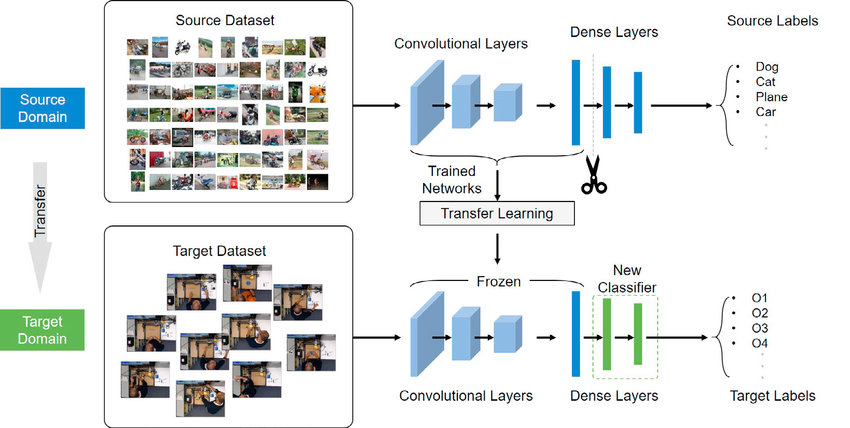
\includegraphics[width=1\textwidth]{images/transfer-learning.png}
    \centering
    \caption[Comparativa entre un entrenamiento normal y por TL.]
    {Comparativa entre un entrenamiento normal y por TL\protect \cite{transfer-learning}.}
    \label{transfer-learning}
\end{figure}

A diferencia del entrenamiento convencional, TL permite que las 
capas iniciales del modelo —en este caso, las capas 
convolucionales— permanezcan congeladas, conservando así el 
conocimiento pre-aprendido del conjunto de datos original. 
Posteriormente, se agregan nuevas capas densas, similares a 
un perceptrón multicapa (MLP), que funcionan como clasificadores 
específicos para la nueva tarea. De esta forma, solo las capas 
finales requieren entrenamiento, lo que reduce la cantidad de 
datos necesarios y mejora la precisión. Este procedimiento, 
conocido como ``\textit{fine-tuning}'', ajusta el aprendizaje 
previo para adaptarlo a un conjunto de datos diferente, 
ahorrando tiempo y recursos computacionales, además de obtener 
mejores resultados que un entrenamiento regular.

\subsection{\textit{Pipelines} actuales para la clasificacion de violencia}

La literatura actual muestra un creciente interés en la 
detección automática de violencia en videos mediante la 
combinación de redes convolucionales (CNN) y redes de 
memoria a largo plazo (LSTM) \cite{sudhakaran2017learning}. 
Las CNN se utilizan para extraer características espaciales 
relevantes de los fotogramas, permitiendo identificar 
patrones visuales y contextos que podrían indicar situaciones 
violentas. Posteriormente, estas características son procesadas 
por las LSTM, las cuales se encargan de capturar la dinámica 
temporal y las dependencias de largo plazo entre los 
fotogramas, mejorando la capacidad de detectar eventos 
violentos que se desarrollan a lo largo del tiempo.\\

En diversos estudios se ha demostrado que la integración 
de ambas arquitecturas permite explotar de forma sinérgica 
las ventajas de cada una \cite{mohammadi2022cnn}: las CNN fortalecen la comprensión 
del contenido visual a nivel de detalle y textura, mientras 
que las LSTM aportan una perspectiva temporal que es crucial 
para identificar patrones de comportamiento complejos y 
secuenciales propios de la violencia. Este tipo de 
\textit{pipeline} ha sido evaluado en diferentes escenarios, 
incluyendo videos de vigilancia y grabaciones deportivas, 
logrando así mejores tasas de detección en comparación con 
métodos que utilizan únicamente análisis espacial o temporal 
de manera aislada.\\

Un claro ejemplo de lo mencionado anteriormente, 
es el artículo de Jeff Donahue
\cite{Donahue2016}. Su investigación se centra en el 
desafío de trabajar con datos visuales que contienen 
información espacial y temporal. La idea central es 
integrar ambas arquitecturas en un único sistema 
end-to-end: las CNNs se encargan de extraer 
representaciones ricas de contenido visual, y las 
LSTMs modelan la dinámica secuencial, permitiendo 
aplicaciones en reconocimiento de actividades en video y 
generación de descripciones de imágenes. \\

Entre sus principales contribuciones, este trabajo 
logró sentar las bases en la integración de 
arquitecturas visuales y secuenciales. Su enfoque ha 
influido en numerosos trabajos posteriores en áreas como 
la descripción automática de videos, el análisis de 
secuencias complejas y el desarrollo de modelos más 
integrados para tareas multimodales.\\

Utilizando esta lógica, se encuentran trabajos\cite{Orozco2021} en los que 
destacan la efectividad de estas estrategias al combinar 
etapas de preprocesamiento, extracción de características 
espaciales mediante CNN, y análisis secuencial temporal con 
LSTM. Asimismo, se discuten los desafíos asociados a la 
variabilidad de escenarios y la detección en tiempo real, 
aspectos que continúan motivando la investigación y 
optimización de estos sistemas. Como resultado final de su 
experimentación, los autores lograron un F1-score de 91\% 
lo cual indica que fue \textit{pipeline} robusto el 
problema que intentó resolver basado en la clasificación de 
acciones humanas basado en videos. Los \textit{pipelines} híbridos 
basados en CNN y LSTM representan una tendencia robusta en 
el campo de la detección de violencia, contribuyendo 
significativamente a la mejora en la precisión y eficiencia 
de los sistemas de análisis de video.\\

Otro artículo que también utiliza esta misma lógica es el de
Swathikiran Sudhakaran and Oswald Lanz \cite{Sudhakaran2017}. Su objetivo consistió 
en el mismo del presente trabajo, la detección de violencia. 
Para ello, se utilizó el \textit{dataset} de Hockey Fights, 
el cuál contiene videos de eventos violentos en partidos de 
hockey. Este \textit{dataset} es bastante usado como \textit{benchmark} 
y consiste de un conjunto de imágenes etiquetadas de manera 
homogenea. La variación más significativa que realizaron fue el 
uso de celdas convLSTM en vez de LSTM regulares para poder 
obtener un \textit{accuracy} más elevado. Con su \textit{pipeline} 
lograron obtener una \textit{accuracy} de 97\%, generando un 
nuevo record para este \textit{benchmark} y marcando un nuevo 
estado del arte. \\

De la misma manera y utilizando el mismo \textit{dataset} de 
Hockey Fights, se encuentra el trabajo de Al-Maamoon R. Abdali 
y Rana F. Al-Tuma \cite{Abdali2019}. Ellos se basaron en el 
trabajo anteriormente mencionado para su implementación. 
Para ello, utilizaron la misma configuración del 
\textit{pipeline} pero incluyeron capas 
conv3d y 40 celdas para el aprendizaje de la LSTM sin ser 
convolucionales. Utilizando aquella configuración logrando 
obtener un \textit{accuracy} de 96.33\% 
pero al mismo tiempo obteniendo una mejora de 4 veces en la 
velocidad (representado en el número de fps), representando 
una mejora del estado del arte en su tiempo al mantener el 
mismo nivel de \textit{accuracy} pero mejorando el 
\textit{performance}.\\

El último artículo a revisar es el de Patel Mann 
 \cite{Mann2021}. En su trabajo utilizó Resnet50, InceptionV3 
y VGG19 como extractores de características. En cambio, 
utilizaron solo una celda LSTM para la clasificación y como 
resultados obtuvieron 90\% de precisión para 
el dataset de Hockey fights, representando una disminución a 
comparación de los anteriores trabajos, aunque permitió optimizar 
el uso de memoria sin perder drásticamente el \textit{performance} 
de todo el \textit{pipeline}.\\

Como se puede ver, el \textit{pipeline} CNN-LSTM propuesto ha 
sido utilizado a lo largo de los últimos años para resolver 
problemas similares e iguales al nuestro. En ese sentido nos hace 
sentido tratar de extender la aplicación de este y optimizarlo 
para tratar de ver como es que diferentes configuraciones del 
mismo permiten mejorar ya sea el \textit{performance} o el 
\textit{accuracy} de la propuesta.
